\documentclass[projektplan/plan.tex]{subfiles}

\begin{document}
\section{Fasplan}
Fasplanen beskriver grovt de aktiviteter som ingår i de olika faserna och ger
en översikt på projektfaserna.
\subsection{Under projektet}
Under projektets gång kommer en del aktiviteter tas hand om. De flesta är
implementationer eller hårdvarukopplingar mellan flera hårdvarukomponenter.
\subsubsection*{Utbildning}
Lära sig hur man använder mjukvaror som exempelvis OpenCV, AVR, KiCAD etc.
Inlärning av hur OS-Raspberry funkar och andra teoretiska delar angående
mikrodatorerna samt överföringsprotokollen måste göras.
\subsubsection*{Kamera}
En kamera ska monteras på chassit, kopplas samman med mikrodatorn i
kommunikationsmodulen.
\subsubsection*{Kommunikation mellan moduler}
Intermodulär kommunikation ska implementeras så flera moduler kan kommunicera
med varandra.
\subsubsection*{Bildbearbetning}
Bilddata från kameran ska bearbetas med OpenCV och bilddatan tolkas till
relevant data.
\subsubsection*{Bearbeta sensorvärden}
Sensorvärdena ska bearbetas och värdena ska tolkas till relevant data.
\subsubsection*{Filtrera ner spänning}
Eftersom mikrodatorns GPIO (general-purpose input/output) pinnar max kan ta
emot 3.3V måste ett filter skapas för att filtrera ner spänningsnivån från 5V
till 3.3V.
\subsubsection*{Aktivera motor}
Skicka styrparametrar från styrmodulens processor till motorn och få den att
driva hjulen.
\subsubsection*{Rotera svängaxel}
Skicka styrparametrar från styrmodulens processor till motorn och få den att
rotera svängaxeln.
\subsubsection*{Bromsa genom att backa}
Försöka skicka styrmoduler till motorn och få den att driva hjulen bak
samtidigt som hjulen rullar framåt för att imitera bromsning.
\subsubsection*{Reglera körning}
Implementera reglering av körning så bilen tar hänsyn till vägmarkeringar och
inte kör av vägen.
\subsubsection*{Pulsbreddsmodulering (PWM)}
Implementera pulsbreddsmodulering så att hastigheten till motorerna kan
justeras.
\subsubsection*{Databuss}
Bestäm vilket överföringsprotokoll som ska användas för databusar, samt
implementera databussar.
\subsubsection*{Kretsschema}
Designa, rita och konstruera kretsscheman till styrmodulen, sensormodulen samt
kommunikationsmodulen. KiCAD kan användas för att rita kretsscheman.
\subsubsection*{Sensorvärden}
Behandling av värdena sensorerna ger ut måste ske. Värdena sensorerna ger måste
filtreras från brus, därefter kan de användas för att indikera objekt på vägen.
Därefter ska sensorvärdena skickas till kommunikationsmodulen.
\subsubsection*{Bärbar dator}
En trådlös länk mellan mikrodatorn och en bärbar dator måste sättas upp. Ett
gränssnitt för att kommunicera med mikrodatorn via den bärbara datorn ska
skapas. Användaren ska kunna mata in en karta till gränssnittet och
gränssnittet ska kunna visa bilens position på kartan.


\subsection{Efter projektet}
Vissa aktivitetar sker efter projektet och beskrivs i grova drag i det här
avsnittet.
\subsubsection*{Levererans}
Den färdiga produkten ska levereras till beställaren efter konstruktionens
slut. Ett acceptanstest görs med beställaren så att beställaren är nöjs med den
levererade produkten. En tekniskt dokumentation och en användarhandledning ska
skickas till beställaren. Hårdvaran ska återlämnas till ISY efter
konstruktionens slut.
\subsubsection*{Efterstudie}
Reflektion och återkoppling av projektet ska göras och lämnas in till
beställaren efter projektets slut. Analys av arbete och problem, samt vad
projektgruppen har uppnåt under projektets gång. En sammanfattning av viktiga
erfarenheter och goda råd till liknande projekt ska inkluderas i efterstudien.

\section{Organisationsplan för hela projektet}

\begin{figure}[h]
    \centering
    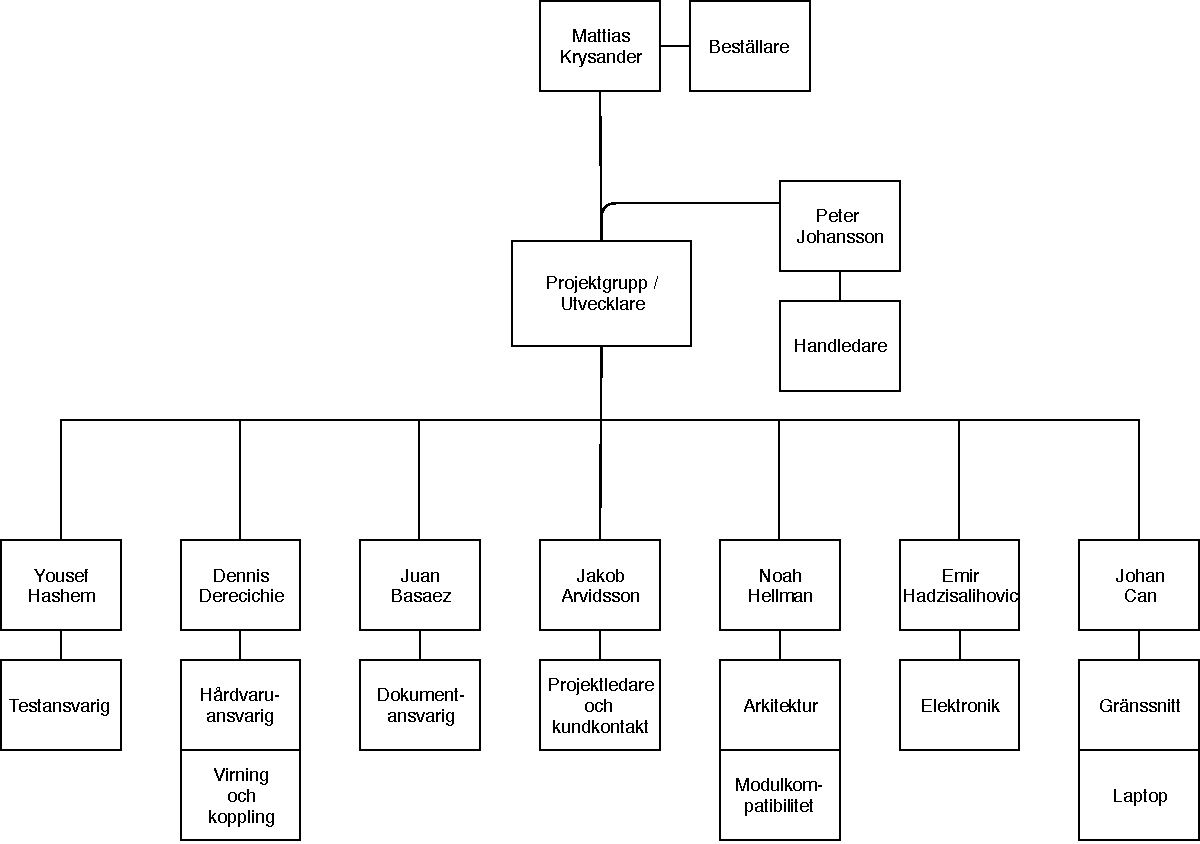
\includegraphics[width=0.6\linewidth]{projektplan/figures/orgplan.pdf}
    \caption{Övergripande bild över organisationsstrukturen}
    \label{fig:orgplan}
\end{figure}

Här beskrivs hur gruppen kommer att organisera arbetet under projektets gång.
Bland annat är planen att gruppen ska sträva efter att dela upp arbetet till
små grupper. Eftersom det finns tre moduler så är själva planen att gruppen
delas upp i tre grupper där vardera grupp arbetar med sin egen modul. Vid
kritiska delar, t.ex där alla moduler är beroende till att något ska vara
färdigt så ska gruppen tillsammans lösa detta. Om en grupp stöter på hinder
så ska gruppen hjälpas åt att tillsammas lösa problemet.

\newpage
\subsection{Villkor för samarbetet inom projektgruppen}
\label{sec:doc}
Nedan följer en lista av de punkter gruppen har enats om att följa vid samarbete.
{\renewcommand{\arraystretch}{1.6}
\begin{longtable}{p{0.8\textwidth}p{0.15\textwidth}}
    \bfseries Fråga &
    \bfseries Inställning \\\hline
    Deltagarna i gruppen ska gemensamt göra upp ordningsregler för gruppen om
    tider, närvaro, förberedelse etc. &
    Instämmer helt
    \\
    Alla deltagare i gruppen ska delta vid de tillfällen som gruppen kommit
    överens om. &
    Instämmer helt
    \\
    Alla deltagare i gruppen ska komma väl förberedda till sammankomsten. &
    Instämmer delvis
    \\
    Det är viktigt med en ”samordnare” i gruppen. &
    Instämmer helt
    \\
    Arbetsuppgifterna ska fördelas likvärdigt mellan gruppmedlemmarna, så att
    tid- och arbetsinsatsen blir ungefär lika stor. &
    Instämmer helt
    \\
    När vi arbetar i gruppen ska vi hålla oss till fakta och undvika prat om
    känslor och personliga erfarenheter. &
    Instämmer delvis
    \\
    Samarbetet i gruppen måste när som helst kunna diskuteras öppet, även om
    det innebär obehag för någon. &
    Instämmer helt
    \\
    Den som inte bidrar aktivt ska inte heller dra nytta av gruppens gemensamma
    arbete. &
    Instämmer delvis
    \\
    Det är viktigt att ge varandra återkoppling, såväl positiv som negativ. &
    Instämmer helt
    \\
    Varje träff avslutas med en utvärdering, där var och en belyser hur arbetet
    i gruppen fungerat. &
    Tar helt avstånd
    \\
    Vår grupps ambitionsnivå är att arbetet ska leda till att det framtagna
    resultatet i projektet blir det bästa tänkbara. &
    Instämmer delvis
    \\
    
    \endhead
\end{longtable}}

\noindent
\newpage
\subsection{Definition av arbetsinnehåll och ansvar}
Vad som anses vara en bra arbetsinsats definieras av majoriteten i gruppen.
Ansvar i gruppen är att man ska vara ärlig mot varandra och vid begäran ge en 
ärlig återkoppling om hur arbetet har gått. Om man står för en viss
konstruktion som inte fungerar så bär man ansvaret att se till att informera
gruppen. Därefter har man ansvar att rätta felet eller att be om hjälp där
man ska föklrar hur konstruktionen är tänkt att fungera.
\end{document}
